\documentclass{clase/sipa}

%===========================================================
% External packages
%===========================================================
\usepackage[version=4]{mhchem}

%===========================================================
% Congress Number, Name and Date; and proceedings' authors
%===========================================================

\numero{13}
\titulo{Semana Internacional en Producción Agropecuaria}
\titulocorto{SIPA}
\fecha{del 7 al 11 de septiembre de 2026}
\titulodos{Conferencias magistrales, resúmenes, cursos y conversatorio}

% Name between {} to avoid problems with the code, and orcid ID
% The code is structured to work regardless of whether you include an Orcid ID or not
\authors{
  {e.g. This name doesn't have an Orcid},;
  {Véliz Romero, Francisco},0000-0002-3456-7890;
}

% PDF  metadata
\hypersetup{
	pdftitle={Memorias de la \eventnumber\space\eventtitle: \eventsubtitle},
	pdfauthor={Véliz-Romero Francisco Gerardo},
	pdfproducer={LaTeX with TeXworks},
	pdfcreator={Véliz-Romero Francisco Gerardo},
	pdfcreationdate = {D:20261002},
	pdfmoddate = {D:20260930},
	pdflang = {es-MX},
	pdfsubject = {XIII SIPA},
	pdfkeywords = {XIII; SIPA; memorias}
}

%===========================================================
% Pagestyle and other stuff
%===========================================================

% Forces a pagestyle in all TOC
\tocloftpagestyle{preindex}
%\raggedbottom

\begin{document}

%===============================================================================================
% Pre table of contents section
%===============================================================================================

% Additional content in the proceedings, including information about the committees
% established for the event, the congress program and more
\newpage
%===============================================================================================
% Event's programs, information or other content
%===============================================================================================

% It's important to include "\hoffset=0pt"
% before including PDF's or other additional files, as the "\setlength{\hoffset}{-0.5in}"
% in the .cls moves all the included files to the left
{\hoffset=0pt
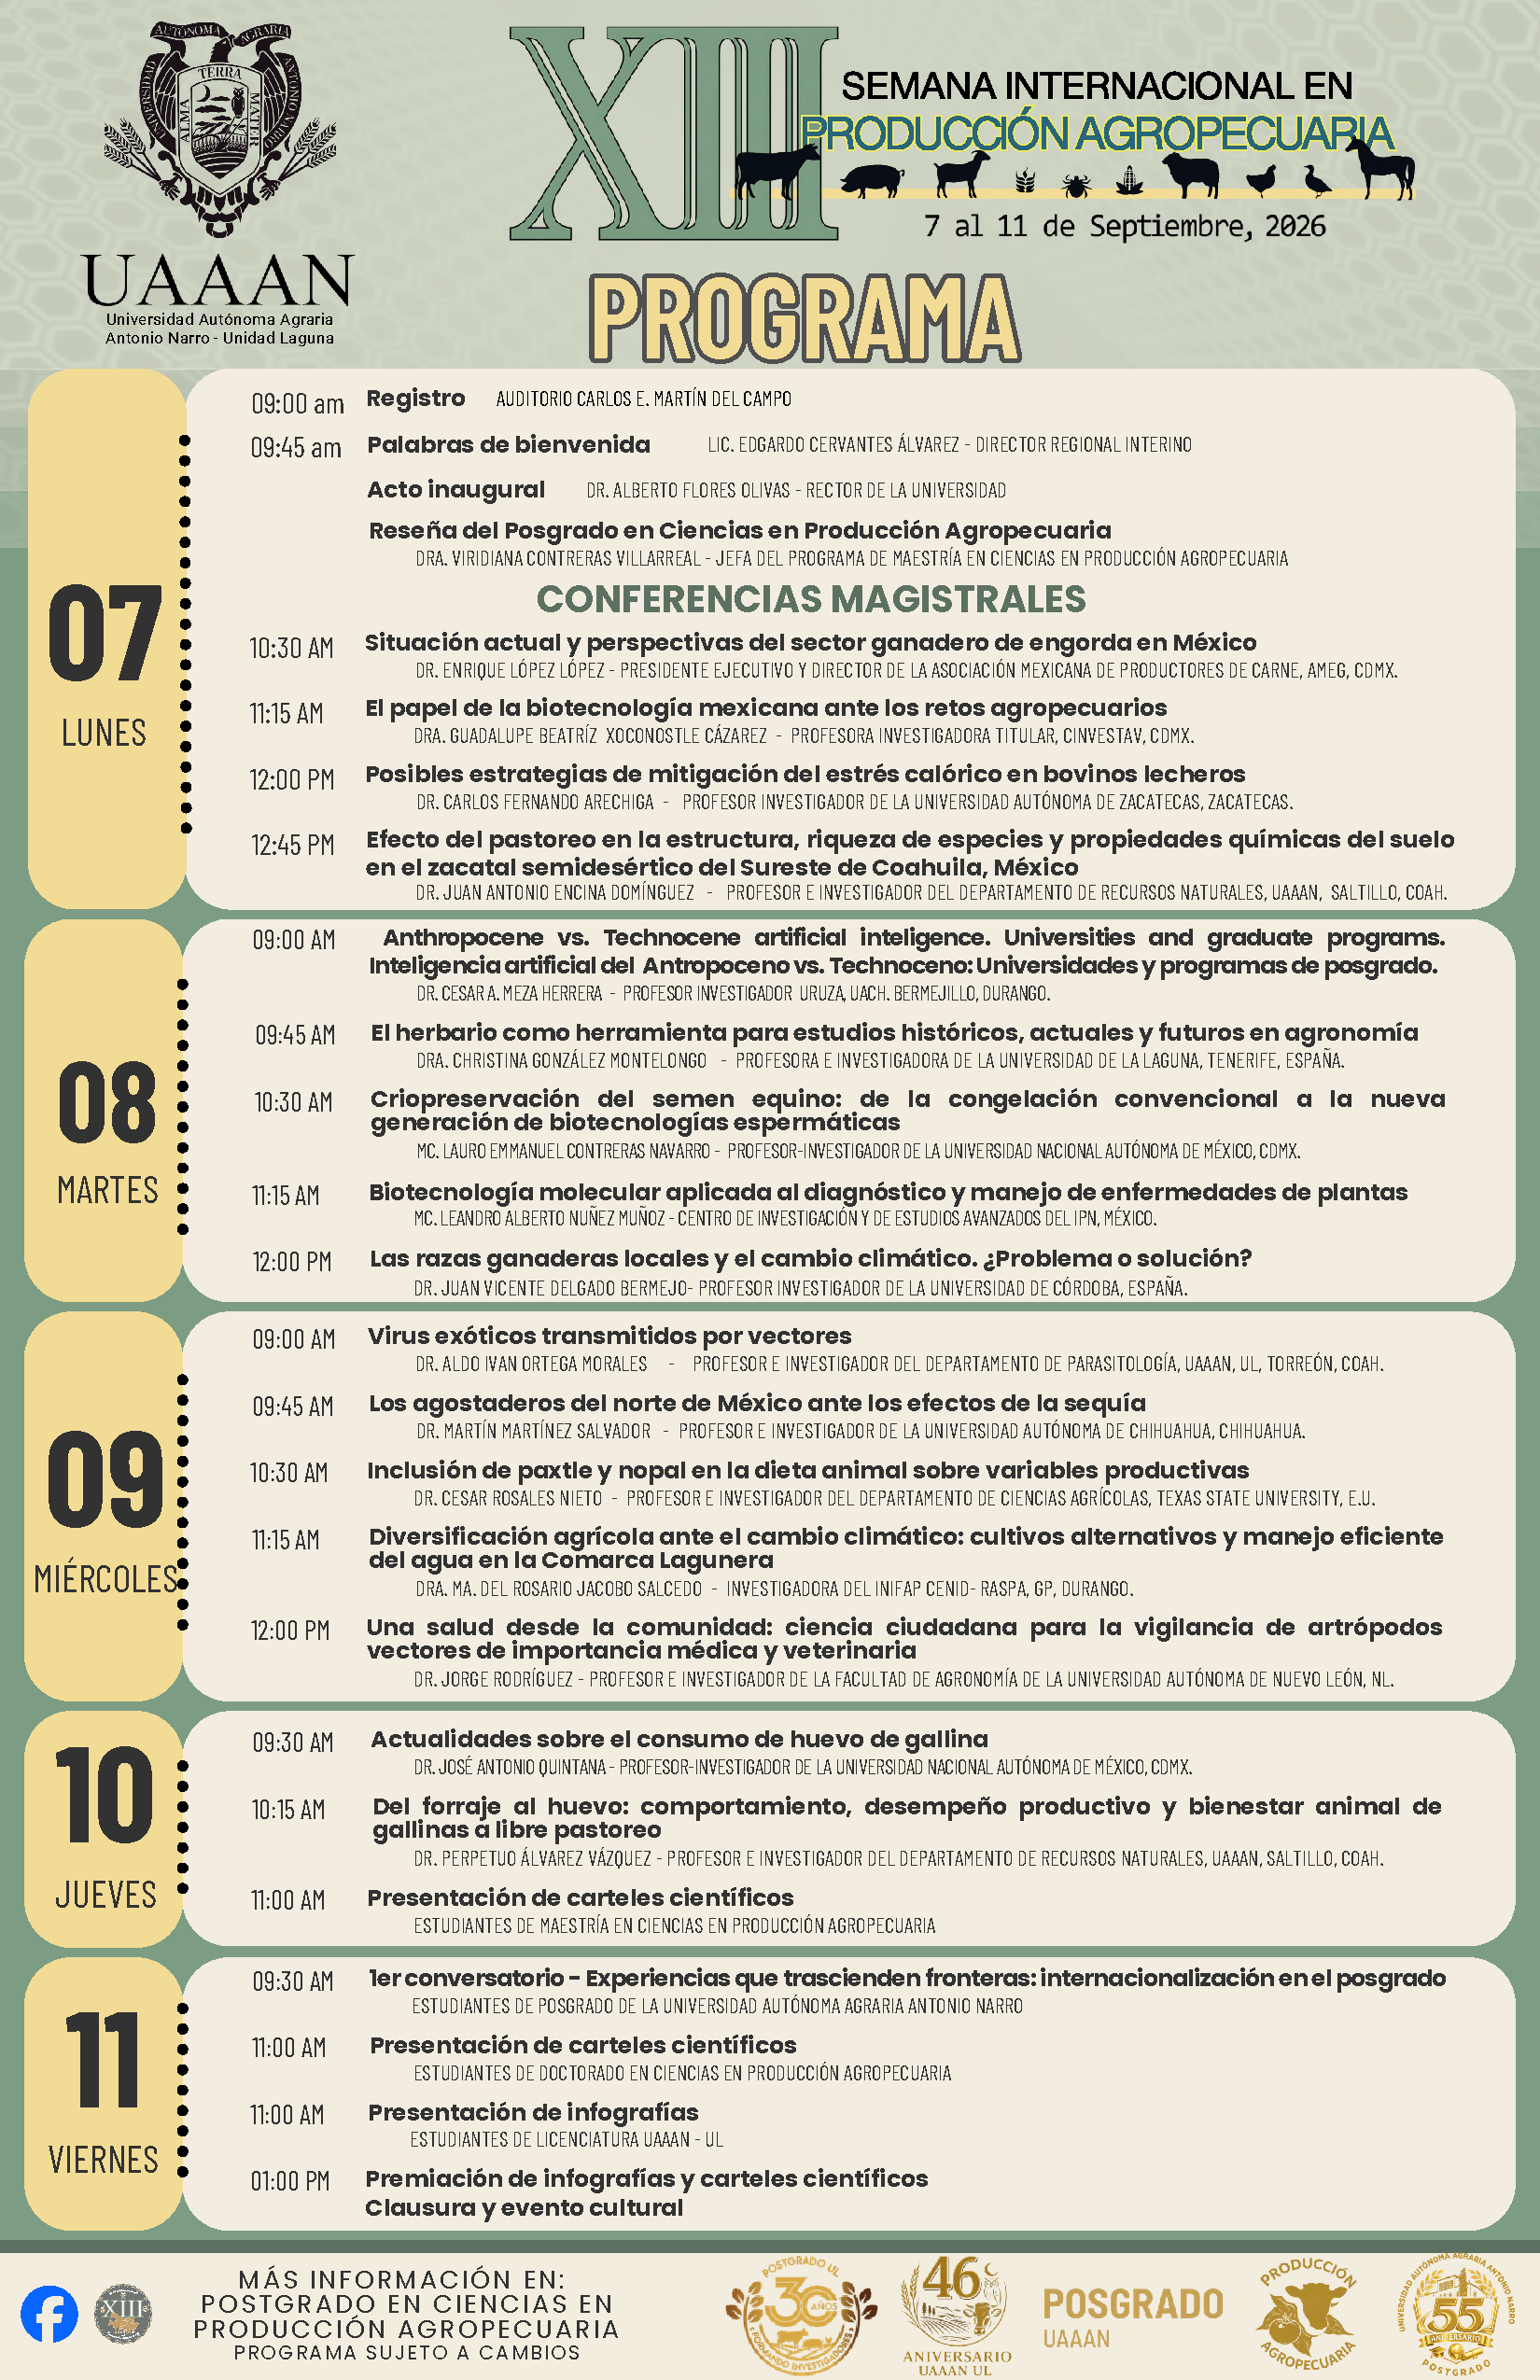
\includepdf[fitpaper=true,pages=-,width=\paperwidth]{images/events/sipa xiii program.pdf}
}

{\hoffset=0pt
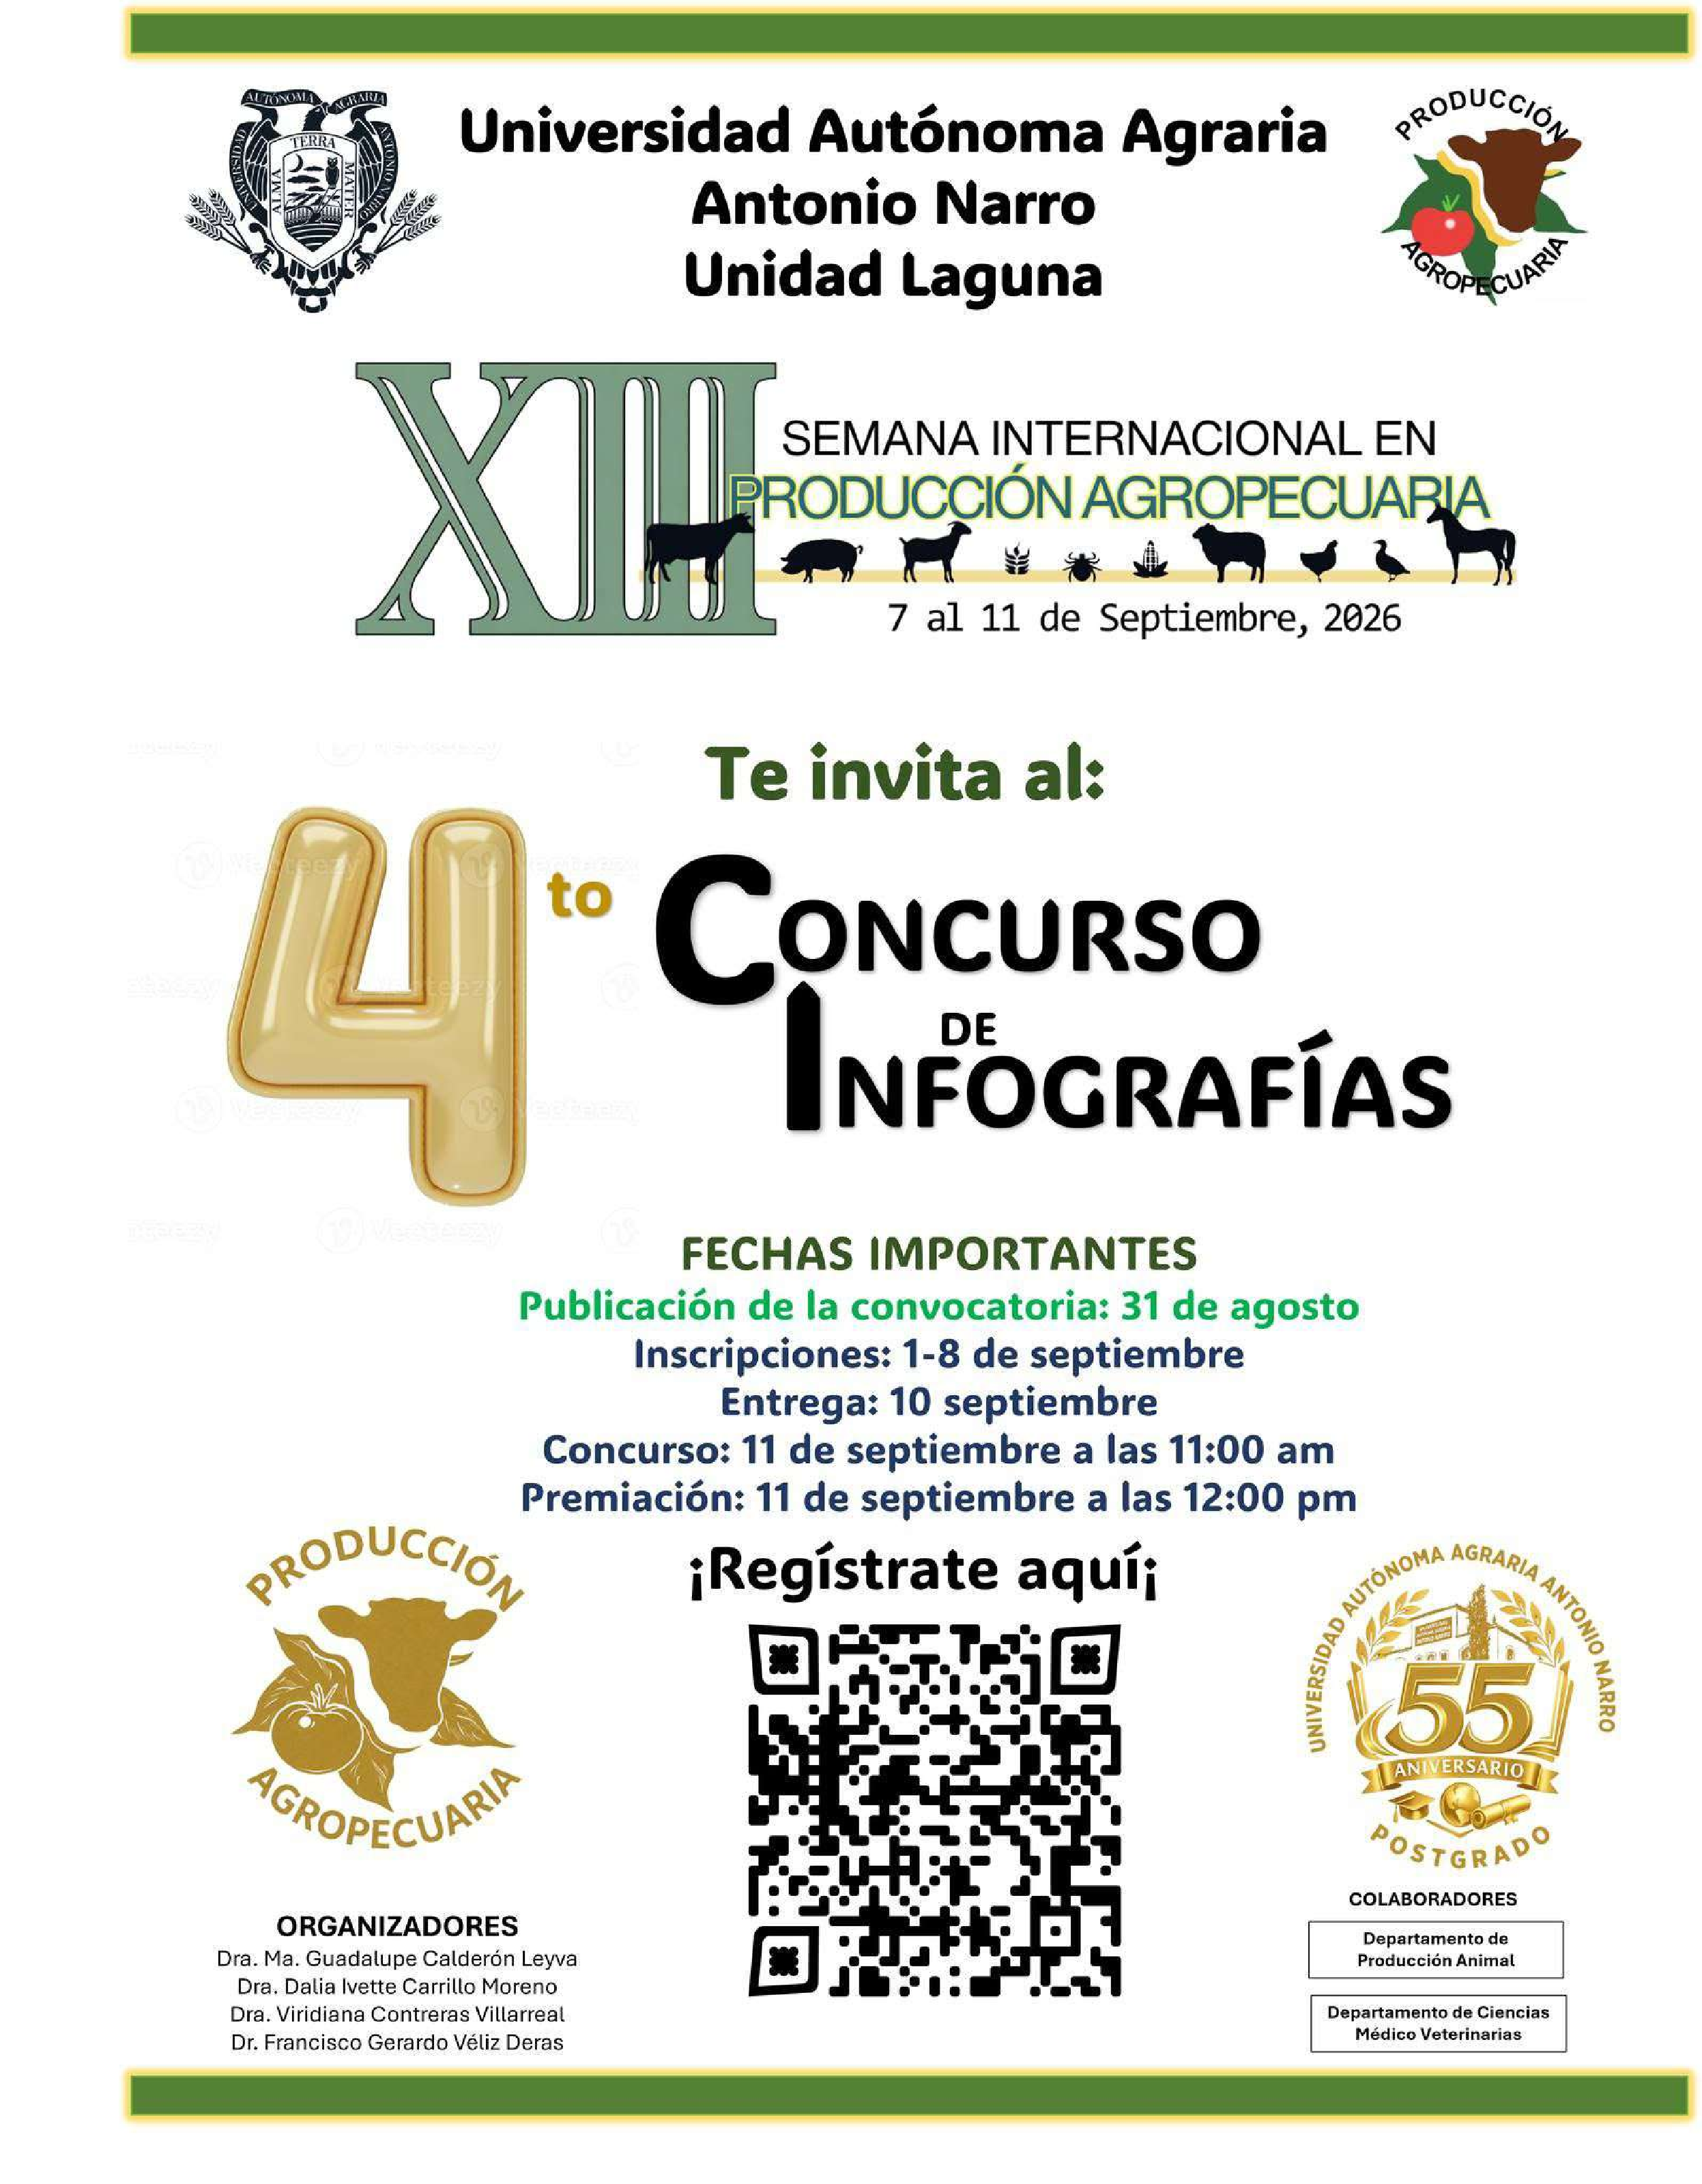
\includepdf[fitpaper=true,pages=-,width=\paperwidth]{images/events/sipa xiii infographics.pdf}
}

%======================
% Geometry
%======================

% Sets new geometry
\bookbodygeometry

% Set roman page numbering, custom page format and page number
\pagenumbering{roman}
\pagestyle{preindex}
% Sets the new page counter, as the included content above wont be classified as pages
\setcounter{page}{5}

%===============================================================================================
% Event's ntroduction
%===============================================================================================

\subseccion{Introduction}

\blindtext

\raggedleft
Lic. Francisco Gerardo Véliz Romero\\[1mm]
\textit{Estudiante de Maestría en ciencias en Producción Agropecuaria}\\[1.5mm]
\small{Adidtional info you could add?}

\raggedright

%===============================================================================================
% Event's organizational chart
%===============================================================================================

\newpage
\subseccion{Event's directory}
% vspace to center content in the middle of the page
\vspace*{\fill}
\begin{center}
	\fontsize{13}{16}\selectfont
	
	\textbf{Rector}
	
	X\\[1.8cm]
	
	\textbf{Director Regional}
	
	X\\[1.8cm]
	
	\textbf{Subdirector de Postgrado}
	
	X\\[1.8cm]
	
	\textbf{Jefe del Departamento de Postgrado}
	
	x\\[1.8cm]
	
	\textbf{Jefe del Programa de Maestría}
	
	x\\[1.8cm]
	
	\textbf{Jefe del Programa de Doctorado}
	
	X\\[1.8cm]
	
\end{center}
% vspace to center content in the middle of the page
\vspace*{\fill}

%===============================================================================================
% Organizing committees
%===============================================================================================

\newpage

% Forces columns centering even with inner-column separation
% Code to remove separation (though you'll have to declare it again to restore it again)
%\setlength{\columnsep}{0pt}
\makebox[\textwidth][c]{%
\begin{minipage}{1.1\textwidth}
\begin{multicols}{2}
[\subseccion{Comités}\vspace*{1cm}]
\centering
\vspace*{-.8cm}
\subtitulos{Organizing Chairman}
X
\subtitulos{Organizing Commitee}
X
\subtitulos{Technich commitee}
X
\subtitulos{Proceedings edition's commitee}
X
\end{multicols}
\end{minipage}
}

\newpage
%\setlength{\columnsep}{3pt}
\makebox[\textwidth][c]{%
\begin{minipage}{1.1\textwidth}
\begin{multicols}{2}
[\subseccion{Comités}\vspace{.3cm}\subtitulos{Poster's evaluation commitee}\vspace*{.5cm}]
\centering
X

X

X

X

X

X
\end{multicols}
\end{minipage}
}


\newpage
% Content unused in the proceedings
\subseccion{National Speakers}

\bandera{}
\confname{Lic. Francisco Gerardo Véliz Romero}
\confsch{Universidad Autónoma Agraria, Unidad Laguna}
\conffac{}
\confjob{Estudiante de Maestría \href{https://orcid.org/0009-0008-5154-9067}{\aiOrcid}}
\confimgone{images/speakers/Lic. Francisco Gerardo Véliz Romero}
\confimgtwo{images/speakers/logo uaaan}
\conftext{4}{3}{1}{%
	\blindtext\\
	\blindtext
}

\conference

\bandera{NG}
\confname{Dr. Abiodum Eunice Adefemisoye}
\confsch{Universidad Autónoma Agraria Antonio Narro, Unidad Laguna}
\conffac{Departamento de Producción Agropecuaria}
\confjob{Estudiante de Doctorado \href{https://www.researchgate.net/profile/Abiodun-Eunice-Adefemisoye-2}{\aiResearchGate}}
\confimgone{images/speakers/Dr. Abiodum Eunice Adefemisoye}
\confimgtwo{images/speakers/logo posgrado}
\conftext{3}{4}{1}{%
	In fact, the way this block it's constructed allows you to customize the text in a broader way. For example, you can write the keynote's lecture title and date\\\\% Here double line break to get the {3} lines stated in the function
	{\large\textbf{Impacto de técnicas de cocción en bioaccesibilidad de fenoles totales en jalapeños meidante digestión gastrointestinal \textit{in vitro}}}\\
	September 11, 2026
}

\conference

\newpage
\subseccion{International Speakers}

\bandera{MX}
\confname{Lic. Francisco Gerardo Véliz Romero}
\confsch{Universidad Autónoma Agraria Antonio Narro, Unidad Laguna}
\conffac{Departamento de Postgrado en Ciencias en Producción Agropecuaria}
\confjob{Estudiante de Maestría \href{https://scholar.google.com/citations?user=9EwJ9GkAAAAJ&hl=es&oi=ao}{\aiGoogleScholar}}
\confimgone{images/speakers/Lic. Francisco Gerardo Véliz Romero}
\confimgtwo{images/speakers/logo posgrado ul 30}
\conftext{3}{5}{1}{%
	Now, this block was created for the proceeding book, but at the end it was decided that a more minimalist design fitted better the proceedings\\
	\blindtext\\
	\blindtext
}

\conferenceone

\bandera{MX}
\confname{Lic. Francisco Gerardo Véliz Romero}
\confsch{Universidad Autónoma Agraria Antonio Narro, Unidad Laguna}
\conffac{Departamento de Postgrado en Ciencias en Producción Agropecuaria}
\confjob{Estudiante de Maestría en Ciencias en Producción Agropecuaria}
\conftitl{This block in specific allows you to print the block even whith missing data, without leaving empty lines}
\confimgone{images/speakers/Lic. Francisco Gerardo Véliz Romero}
\confimgtwo{images/speakers/logo posgrado ul 30}

\conferencetwo

% Codes to print the link and logos for Google Scholar, ResearchGate and Orcid
%\href{https://scholar.google.com/citations?user=}{\aiGoogleScholar}
%\href{https://www.researchgate.net/profile/}{\aiResearchGate}
%\href{https://orcid.org/}{\aiOrcid}


%===============================================================================================
% Table of contents
%===============================================================================================

% For some reason, the TOC didnt allow me to change the title's format
% The following code forces TOC to stop resetting the aforementioned format
\newpage
\begingroup

\makeatletter
% TOC custom name
\renewcommand{\contentsname}{Content}
% Function to force the TOC's name change
\renewcommand{\tableofcontents}{%
  \if@twocolumn
    \@restonecoltrue\onecolumn
  \else
    \@restonecolfalse
  \fi
  \subseccion{\contentsname}%
  \@starttoc{toc}%
  \if@restonecol\twocolumn\fi
}
\makeatother

% Forces TOC to be sided to the left, as for some reazon, the text was justificatedin my document
\parshape 0
\raggedright
\tableofcontents

\endgroup

%===============================================================================================
% Post table of contents section
%===============================================================================================

%=================================================
% Keynote lectures section
%=================================================

\newpage
\pagestyle{posindex}
\pagenumbering{arabic}

% This function is key to the proceedings header
% "no" allows you to place the Author's name in the header
% "yes" leaves a blanc spaceto write the section custom title
\pagenblanc{alone}
% Forces justified text without extreme white spaces, though some ugly spacing still appears
%\sloppy
\justifying
\part{Keynote lectures}

\newpage
\subseccion{Conferencista Internacional}

%\vspace{-0.5cm}
%\subtitulos{Conferencista Internacional}
%===============================================================================================
%								6ta conferencia (internacionales)
%===============================================================================================

\bandera{ES}
\confname{Dra. Cristina González Montelongo}
\confsch{Universidad de La Laguna}
\conffac{}
\confjob{Profesora e investigadora\, \href{https://orcid.org/0000-0001-9236-890X}{\aiOrcid}\, \href{https://www.facebook.com/paulino.aguilar.7568596/videos/1092630373338066/}{\faTv}}
\confimgone{images/speakers/Dra. Cristina González Montelongo}
\confimgtwo{images/speakers/logo ull}
\conftext{4}{3}{1}{%
	La Dra. Cristina González Montelongo es bióloga con Máster Universitario de Biodiversidad Terrestre y Conservación en Islas, y Doctora por la Universidad de La Laguna. En 2012 se inició en la investigación botánica a través de una Beca de Colaboración, que dio paso a dos Proyectos de Innovación Educativa.  Ha alternado sus estudios de máster con el trabajo para empresas del sector medioambiental. Permitiéndole desarrollar actividades de educación ambiental, informes de impacto ambiental, Seguimientos de Especies Amenazadas (SEGA), actualización de las bases de datos de especies silvestres y de especies amenazadas del Gobierno de Canarias, entre otras actividades. Su tesis doctoral se centró en el estudio del monteverde canario empleando los líquenes epífitos como organismo modelo. Estos estudios los alternó con el trabajo como técnico en el Herbario TFC (Herbario Institucional de la ULL, SEGAI), encargándose desde entonces del mantenimiento del mismo y su informatización, además de facilitar mejoras en la gestión de las colecciones y en las propias instalaciones, sin abandonar en ningún momento las actividades de divulgación, docencia (reglada y no reglada), investigación y asesoramiento técnico a investigadores y empresas del sector medioambiental, a través de su trabajo en el Herbario TFC. Su trabajo e investigaciones han resultado en 8 informes científico-técnicos, 14 artículos científicos, 1 artículo de divulgación científica, más de 30 contribuciones a congresos nacionales e internacionales y más de 30 participaciones en ferias, festivales y jornadas de divulgación, además de haber organizado un congreso científico y dos jornadas técnicas. Es Personal Técnico de Apoyo en el Servicio Herbario TFC del SEGAI, y miembro del grupo de investigación “Liquenología” del Departamento de Botánica, Ecología y Fisiología Vegetal. Actualmente, colabora con numerosos equipos de investigación y proyectos tanto de la ULL como nacionales e internacionales.%
}

\conference

\newpage
\begin{refsection}
\pagenblanc{no}
\begin{wrap}
	\chapter{Francisco Véliz}
	% If you're using TexStudio, this line helps you to identify the keynote/document/course in the editor's TOC
\end{wrap}
\cero
\abbrevnombs{Véliz-Romero}{Francisco}{Francisco-Gerardo}{Gerardo}
\tocauthor{Véliz-Romero Francisco Gerardo}% This function adds the name in the TOC
\author{%
	Véliz-Romero Francisco Francisco-Gerardo Gerardo
}
\ijaffiliation{%
	Asociación Mexicana de Productores de Carne AMEG, A. C.
}
% In the first {} you can add any text, and the second {} the email
% The function adds automatically an space between both items
\corresponding{Este es un ejemplo:}{exaple@gmail.com}
\title{Keynote's title}

\maketitle

\vspace{.5cm}
\begin{resumen}
	\blindtext
	\blindtext
	\blindtext
\end{resumen}

\keywords{i'll say, maximum four, keynotes, but, it doesn't, have, limits}

% I personally dont need the subsection's title in TOC, so i used the *
\subsection*{The subsection: Of the keynote}

\blindtext[1] \textcite{example}. \blindtext[1]

\blindtext[1] \parencite{example-5}

\subsection*{Other subsection}

\blindtext[1] \parencite{example-2}.

\blindtext[1] \textcite{example-1,example-2} \blindtext[1] \parencite{example-6}.

\subsection*{More sections?}

\blindtext[1]

\begin{itemize}
	\item[a.] \blindtext[1]
	\item[b.] \blindtext[1]
	\item[c.] \blindtext[1]
	\item[d.] \blindtext[1]
\end{itemize}

Altough i used itemize, it sould also support ennumerate environment too, though i havent checked it.

% Adding references that are not printed in the text don't break the document ;)
\nocite{example-3,example-4}

% if you dont want the bibliography title appearing in the toc, you can use "misubseccion"
% If you want the bibliography title appearing in the toc, change it to "subbibintoc"
\printbibliography[heading=misubseccion]
\end{refsection}

\newpage
\pagenblanc{alone}
\subseccion{Conferencista especial}

%\vspace{-0.5cm}
%\subtitulos{Conferencista Especial}

%===============================================================================================
%								Conferencia Especial
%===============================================================================================

\bandera{}
\confname{MVZ. Mario Guevara Acosta}
\confsch{Dirección General de Salud Animal}
\conffac{Comisión México–Estados Unidos para la Prevención de la Fiebre Aftosa y otras Enfermedades Exóticas de los Animales (CPA)}
\confjob{Coordinador Regional de la CPA Región Laguna II\, \href{https://www.facebook.com/share/v/1CghyqfprV/}{\faTv}}
\confimgone{images/speakers/MVZ. Mario Guevara Acosta}
\confimgtwo{images/speakers/logo cpa}
\conftext{4}{3}{1}{%
	\textbf{Generalidades del Gusano Barrenador}\\
	\textit{11 de septiembre de 2026}\\
	El MVZ. Mario Guevara Acosta es egresado de la Universidad Autónoma Agraria Antonio Narro, y ha ostentado el cargo de Profesional Ejecutivo de Servicios Especializados en la Dirección General de Salud Animal del CPA, bajo el Servicio Nacional de Sanidad, Inocuidad y Calidad Agroalimentaria (SENASICA) durante los años 2011 y 2012. En la actualidad, ejerce como Coordinador Regional de la CPA Región Laguna II desde el año 2025, y es presidente del Grupo Estatal de Emergencia en Sanidad Animal (GEESA), conformado por el Gobierno del Estado de Chihuahua. Impartiendo capacitaciónes sobre las medidas de prevención, vigilancia y control del Gusano Barrenador del ganado, así como de los procesos y protocolos que se deben seguir ante una contingencia sanitaria. Como parte de su trabajo como Coordinador Regional de la CPA Región Laguna II, ha realizado conferencias en universidades como la Universidad Juárez del Estado de Durango, la Universidad Autónoma Agraria Antonio Narro y la Unidad Regional Universitaria de Zonas Áridas de la Universidad Autónoma Chapingo, así como  curso-talleres y capacitaciones en la Unión Ganadera Regional de Durango, la Unión Ganadera Regional de Coahuila y la Asociación de Médicos Veterinarios Zootecnistas Especialistas en Bovinos de la Laguna; presentando información sobre el panorama actual del gusano barrenador, así como los riesgos, impactos y estrategias de control y erradicación establecidas para combatir esta problemática sanitaria.%
}

\conference


%=================================================
% Abstracts section
%=================================================

% Abstracts sections
\newpage
\pagenblanc{yes}
% This function clears the previously stablished header's name
\nombsec{}
\part{Posters' abstracts or other content}

\newpage
% Make sections behave as subsections in viewer's- TOC or Browsers
% The first section behaves as the main section
% and all the subsequent sections are labeled as subsections
\begin{browserSubsections}
% Custom section format to make it appear in a sole page
\mychapter{This is a custom chapter}

% Remember to add \newpage  after every \part and \mychapter, or TOC will send you to the previous page
\newpage
\begin{wrap}
	\chapter{Veliz-Romero}
\end{wrap}
\cero
% Given that \pagenblanc{} is set in yes, here will appear the section custom name in the header instead of the abbreviated name
% If you've already declared a section name, you can hide the function to leave it as it is
% If you want to change it, unhide the function and place another name
\nombsec{First Section name}% Custom section name
\abbrevnombs{last names}{fist}{names}{}
\tocauthor{Véliz-Romero Francisco Gerardo}% This function adds the name in the TOC
\author{%
	Véliz-Romero Francisco Gerardo \textsuperscript{1}*,.
	Ramírez-Gottfried Ricardo Israel \textsuperscript{2}
}
\affiliation{%
	1.- Maestría en Ciencias en Producción Agropecuaria -- Universidad Autónoma Agraria Antonio Narro.
	2.- Departamento de Riego -- Universidad Autónoma Agraria Antonio Narro
}
\corresponding{*}{example@gmail.com}
\title{ANÁLISIS DE LA CALIDAD DEL AGUA SUBTERRÁNEA EN PEDRO MEOQUI, CHIHUAHUA, MEDIANTE COMPONENTES PRINCIPALES}

\maketitle

\begin{resumen}
	\blindtext[1]
\end{resumen}

\keywords{calidad del agua, acuíferos, análisis de componentes principales}

\newpage

\begin{wrap}
	\chapter{Other author}
\end{wrap}
\cero
% Given that \pagenblanc{} is set in yes, here will appear the section custom name in the header instead of the abbreviated name
% If you've already declared a section name, you can hide the function to leave it as it is
% If you want to change it, unhide the function and place another name
\nombsec{Second Section Name}% Custom section name
\abbrevnombs{last names}{name}{name}{}
\tocauthor{Véliz-Deras Francisco Gerardo}% This function adds the name in the TOC
\author{%
	Véliz-Deras Francisco Gerardo \textsuperscript{1}
}
\affiliation{%
	1.- Universidad Autónoma Agraria Antonio Narro.
}
\corresponding{}{example@gmail.com}
\title{If you have any scientific name such as (\scientificname{Allobates niputidea}), write it inside the scientificname environment to keep it unchanged}

\maketitle

\begin{resumen}
	\blindtext[1]
\end{resumen}

\keywords{keyword 1, keyword 2, keyword 3}

\end{browserSubsections}

% Make sections behave as subsections in viewer's- TOC or Browsers
% The first section behaves as the main section
% and all the subsequent sections are labeled as subsections
\begin{browserSubsections}
% Custom section format to make it appear in a sole page
\mychapter{This is another custom chapter}

\newpage
\begin{wrap}
	\chapter{Veliz-Romero}
\end{wrap}
\cero
% Given that \pagenblanc{} is set in yes, here will appear the section custom name in the header instead of the abbreviated name
% If you've already declared a section name, you can hide the function to leave it as it is
% If you want to change it, unhide the function and place another name
\nombsec{First Section name for both}% Custom section name
\abbrevnombs{last names}{fist}{names}{}
\tocauthor{Véliz-Romero Francisco Gerardo}% This function adds the name in the TOC
\author{%
	Véliz-Romero Francisco Gerardo \textsuperscript{1}*
}
\ijaffiliation{%
	1.- Universidad Autónoma Agraria Antonio Narro.
}
\corresponding{* Correspondence author:}{example@gmail.com}
\title{Another work}

\maketitle

\begin{resumen}
	\blindtext[1]
\end{resumen}

\keywords{calidad del agua, acuíferos, análisis de componentes principales}

\newpage

\begin{wrap}
	\chapter{Other author}
\end{wrap}
\cero
% Given that \pagenblanc{} is set in yes, here will appear the section custom name in the header instead of the abbreviated name
% If you've already declared a section name, you can hide the function to leave it as it is
% If you want to change it, unhide the function and place another name
%\nombsec{}% Custom section name
\abbrevnombs{last names}{name}{name}{}
\tocauthor{Véliz-Deras Francisco Gerardo}% This function adds the name in the TOC
\author{%
	Véliz-Deras Francisco Gerardo \textsuperscript{1}
}
\ijaffiliation{%
	1.- Universidad Autónoma Agraria Antonio Narro.
}
\corresponding{}{example@gmail.com}
\title{The last work about (\scientificname{Allobates niputidea}), in this whole proceedings}

\maketitle

\begin{resumen}
	\blindtext[1]
\end{resumen}

\keywords{keyword 1, keyword 2, keyword 3}

\end{browserSubsections}


% Although unused, this function changed the indentation of the TOC content
%\addtocontents{toc}{%
%  \protect\setlength{\cftsubsecindent}{3em}%
%}

%=================================================
% Discussion Forum section
%=================================================

\newpage
\pagenblanc{yes}
\nombsec{}
\part{Discussion}

\newpage
% Command to set a chapter's name different in TOC and document
% The first {} is for the chatper's name in TOC
% The second {} is for the chapter's name in the document
% Texorpdfstring write {} as a text in the document and the second {} as bookmark
\begin{browserSubsections}
\mychaptertwo{\texorpdfstring{1er Conversatorio}{1ER CONVERSATORIO}}{1er Conversatorio\\[1cm] Experiencias que trascienden fronteras}

\newpage
{\hoffset=0pt
	
\includepdf[fitpaper=true,pages=-,width=\paperwidth, pages={1,2}]{images/events/sipa xiii discussion.pdf}
}

\newpage
% Command to add a section name, without numbering and dots line in chapter style
% The cirst line edits the indentation of the TOC text
% The second command moves the line to the left, blacknes the text and shortens the distance from the text under it
% The last command restores the indentation of the TOC text
\cftsetindents{section}{0.5cm}{2cm}
\phantomsection
\cftaddtitleline{toc}{section*}{%
	\hspace{0.49cm}\textbf{\MakeUppercase{Experiencias que trascienden fronteras: Internacionalización en el posgrado}}\vspace{-2.5mm}%
}{}
\cftsetindents{section}{1.5cm}{2cm}

\newpage
\begin{wrap}
	\chapter{introduction}
	% If you're using TexStudio, this line helps you to identify the keynote/document/course in the editor's TOC
\end{wrap}

% Adds a section name without printing it in TOC
\phantomsection
\pdfbookmark[0]{\MakeUppercase{Experiencias que trascienden fronteras: Internacionalización en el posgrado}}{}
\section*{\MakeUppercase{Experiencias que trascienden fronteras: Internacionalización en el posgrado}}

\vspace{-0.2cm}
% Name of the section in header
\nombsec{Experiencias que  trascienden: Internacionalización en el posgrado}
% This function adds the name in the TOC
\tocauthor{Ma. Guadalupe Calderón Leyva}
\author{%
	Ma. Guadalupe Calderón Leyva
}
\ijaffiliation{%
	Jefa del postgrado en Ciencias en Producción Agropecuaria
}
\corresponding{}{}
% As no title is placed in this \maketitle, the space is reduced to avoid blanc lines in TOC
\title{\vspace{-5mm}}

% Function to remove the bookmark placed by \maketitle
\begingroup
\ijauthorbookmarkfalse
\maketitle
\endgroup

Un conversatorio es un espacio de diálogo e intercambio de experiencias en el que los participantes comparten experiencias, conocimientos, opiniones y reflexiones sobre un tema en común, generalmente a partir de preguntas orientadoras y con interacción con el público. Tomando en cuenta lo anteriormente dicho, este conversatorio tiene como objetivo generar un espacio de diálogo e intercambio de experiencias sobre estancias académicas internacionales, que permita los estudiantes, tanto internos como externos, conocer de primera mano las oportunidades, aprendizajes y retos de la movilidad internacional, promoviendo una visión global y motivándolos a explorar nuevas oportunidades de formación y colaboración académica.

\begin{table}[H]
	\centering
	\begin{tabular}{cc}
		\multicolumn{2}{c}{\textbf{Schedule}} \\
		\multicolumn{1}{c|}{\multirow{1}{*}{Septiember, 11}} & 9:30 am \\
	\end{tabular}
\end{table}

% Adds the section name in toc without printing the section number
\phantomsection
\section*{PRESENTACIÓN DE AUTORIDADES}
\addcontentsline{toc}{section}{\hspace{-0.1cm}\texorpdfstring{\MakeUppercase{PRESENTACIÓN DE AUTORIDADES}}{\MakeUppercase{PRESENTACIÓN DE AUTORIDADES}}}
\vspace{1.5cm}

\begin{wrap}
	\chapter{Introduction talk}
	% If you're using TexStudio, this line helps you to identify the keynote/document/course in the editor's TOC
\end{wrap}
\cero
% Name of the section in header.
% Given that a fixed name was established for this part of the document, the function can be omited to avoid more changes
%\nombsec{}
% This function adds the name in the TOC
\tocauthor{Dr. Antonio Flores Naveda}
\author{%
	Dr. Antonio Flores Naveda
}
\ijaffiliation{%
	Subdirector de Postgrado -- Universidad Autónoma Agraria Antonio Narro
}
\corresponding{}{}
\title{Introduction talk}

\maketitle
%\vspace{1.3cm}

\newpage
\begin{wrap}
	\chapter{Presentation}
	% If you're using TexStudio, this line helps you to identify the keynote/document/course in the editor's TOC
\end{wrap}
\cero
% Name of the section in header.
% Given that a fixed name was established for this part of the document, the function can be omited to avoid more changes
%\nombsec{}
% This function adds the name in the TOC
\tocauthor{M. C. Alexis Gabriel Pivaral Chávez}
\author{%
	M. C. Alexis Gabriel Pivaral Chávez
}
\ijaffiliation{%
	Estudiante de Doctorado en Ciencias en Producción Agropecuaria
}
\corresponding{}{}
\title{Conoce el Posgrado de la UAAAN: Formación, investigación y oportunidades profesionales}

\maketitle

\vspace*{.5cm}
\begin{resumen}
	\justifying
	El Posgrado de la \textbf{Universidad Autónoma Agraria Antonio Narro (UAAAN)} constituye un espacio de formación especializada, investigación e innovación orientado a atender las necesidades y desafíos del sector agropecuario desde una perspectiva ambiental, social, científica y económica. La institución cuenta con programas de especialidad, maestría y doctorado en diversas áreas de conocimiento relacionadas con las ciencias agrarias, la producción agropecuaria, el manejo sustentable de recursos anturales y el desarrollo e innovación científica y tecnológica; que permiten a los cursantes desarrollar competencias avanzadas para la generación y aplicación de conocimiento. En particular, la \textbf{Maestría y el doctorado en Ciencias en Producción agropecuaria} tienen como propósito formar investigadors y profesionistas especializados en el estudio y atención de problemáticas relacionadas con la producción agrícola y pecuaria, así como la innovación tecnológica y el manejo sustentable de los recursos naturales. La formación de los estudiantes en el programa de \textbf{Ciencias en Producción Agropecuaria} se complementa mediante la participación en proyectos de investigación, seminarios, cursos teórico-prácticos, congresos nacionales e internacionales, y actividades de intercambio académico y científico. Entre estas actividades, destaca la \textbf{Semana Internacional en Producción Agropecuaria}, organizada por el propio programa de posgrado para funjir como un espacio de divulgración, intercambio y vinculación académica, científica y profecional, en donde se presentan los avances y capacidades desarrolladas por los estudiantes, docentes e investigadores del programa. Las principales líneas y áreas de investigación del programa de Posgrado en Ciencias en Producción Agropecuaria abarcan disciplinas relacionadas con la producción agrícola y pecuaria, fitomejoramiento, horticultura, parasitología, biotecnología, recursos naturales, producción vegetal, sanidad agrícola, y apicultura, así como reproducción, nutrición y bienestar animal. Asimismo, estos programas fomentan la vinculación y colaboración con instituciones nacionales e internacionales, ofreciendo oportunidades de movilidad académica con instituciones de América Latina y Europa, y brindando diversas alternativas de desarrollo profesional en los ámbitos académicos, científicos, productivos, empresariales y gubernamentales. En conjunto, la \textbf{Maestría y el Doctorado en Ciencias en Producción Agropecuaria} representan una oportunidad para la formación de profesionistas e investigadores capaces de generar conocimiento, desarrollar soluciones innovadoras, y participar en la atención de los desafíos actuales del sector agropecuario, contribuyendo a su desarrollo y al manejo sustentable de los recursos naturales.
\end{resumen}

\newpage
\begin{wrap}
	\chapter{Semblance}
	% If you're using TexStudio, this line helps you to identify the keynote/document/course in the editor's TOC
\end{wrap}
% Adds a section name without printing it in TOC
\phantomsection
\section*{Discussion forum's semblances}
% Adds the section name in toc without printing the section number
\addcontentsline{toc}{section}{\hspace{-0.1cm}\texorpdfstring{DISCUSSION FORUM'S SEMBLANCE}{DISCUSSION FORUM'S SEMBLANCE}}

\begin{wrap}
	\chapter{Romeo}
	% If you're using TexStudio, this line helps you to identify the keynote/document/course in the editor's TOC
\end{wrap}
% Semblance of the discussion participants
% The main difference between the semblance and the conference blocks, it's that the semblance block only allows the display of the person's own image
% There seems to be a bug only in the first block under a section. this can be solved adding additional lines and rising the space between the text and the image
% Be careful, if you dont add the \\ & \newline, the text will be raised, but the initial paragraph will stay in it's original place
%\phantomsection
%\pdfbookmark[2]{Ing. Romeo Velasco Santiago}{}
\bandera{}
\confname{Ing. Romeo Velasco Santiago}
\confsch{Estudiante de la Maestría Profesional en Tecnología de Granos y Semillas}
\confimgone{images/semblance/sipa xiii semblance 1}
\semblancetext{8}{1}{%
	\vspace{-12mm}%
	\raisebox{-4.5mm}{\\}\newline
	El Ing. Romeo Velasco Santiago, originario del estado de Chiapas, es egresado de la carrera de Ingeniero Agrónomo en Producción, en la Universidad Autónoma Agraria Antonio Narro. Su interés en la producción y mejoramiento de cultivos básicos lo llevó a cursar actualmente la Maestría Profesional en Tecnología de Granos y Semillas en la misma institución. Como parte de su especialización, realizó una estancia internacional en la \textbf{Universidad Federal de Pelotas, en Cap\~ao do Le\~ao, Brasil, Brasil}. Su trabajo actual se centra en la tecnología de semillas y el mejoramiento genético  decultivos resilientes, como girasol y sorgo, orientando sus esfuerzos hacia la seguridad alimentaria y la sostenibilidad agrícola, y cuenta con al menos un artículo publicado sobre el comportamiento agronómico de poblaciones de girasol con alto contenido oleico en el sureste de Coahuila, México.%
}

\semblance

\begin{wrap}
	\chapter{Katherin}
	% If you're using TexStudio, this line helps you to identify the keynote/document/course in the editor's TOC
\end{wrap}
\bandera{CO}
\confname{MVZ. Katherin Castañeda Moreno}
\confsch{Estudiante de la Maestría en Ciencias en Producción Agropecuaria}
\confimgone{images/semblance/sipa xiii semblance 2}
\semblancetext{7}{1}{%
	Katherin Castañeda Moreno es Técnica en Contabilización de Operaciones comerciales y Financieras, Técnica Auxiliar Clínica Veterinaria, Tecnóloga en Producción Ganadera y Médica Veterinaria y Zootecnista, egresada de la \textbf{Universidad Tecnológica de Pereira, Colombia}. Participó en grupos de investigación sobre biodiversidad y conservación, y fue beneficiaria de una peca parcial del Programa de Intercambio Académico Latinoamericano (PILA) en 2023. Ha participado en simponsios y congresos internacionales. Actualmente cursa la Maestría en Ciencias en Producción Agropecuaria en la Universidad Autónoma Agraria Antonio Narro. Sus intereses se enfocan en nutrición y producción caprina, fortaleciendo su formación científica mediante la investigación y el intercambio académico entre Colombia y México.%
}

\semblance

\begin{wrap}
	\chapter{Salomon}
	% If you're using TexStudio, this line helps you to identify the keynote/document/course in the editor's TOC
\end{wrap}
\bandera{}
\confname{Ing. Salomón Isaias Rodríguez Morales}
\confsch{Estudiante de la Maestría en Tecnologóa de Granos y Semillas}
\confimgone{images/semblance/sipa xiii semblance 3}
\semblancetext{7}{1}{%
	El Ing. Rodríguez Morales es originario de Las Rosas, Chiapas, egresado de la carrera Ingeriero Agrónomo en Producción por la Universidad Autónoma Agraria Antonio Narro en el año 2023. Actualmente cursa la Maestría en Tecnología de Granos y Semillas, donde se especializa en la producción y el mejoramietno genético de semillas, particularmente de sorgo y maíz. Su formación profesional incluye una estancia académica en la \textbf{Universidad Federal de Pelotas, en Cap\~ao do Le\~ao, Brasil}, enfocada en tecnología de semillas. Su trabajo se orienta al desarrollo agrícola del país, sustentado en la disciplina, la responsabilidad y el compromiso con la innovación en el sector agropecuario.%
}

\semblance

\newpage
\begin{wrap}
	\chapter{Steffanny}
	% If you're using TexStudio, this line helps you to identify the keynote/document/course in the editor's TOC
\end{wrap}
\bandera{}
\confname{M. C. Steffanny Sánchez Portillo}
\confsch{Estudiante del Doctorado en Ciencias en Agricultura Protegida}
\confimgone{images/semblance/sipa xiii semblance 4}
\semblancetext{7}{1}{%
	Steffanny Sánchez-Portillo es Ingeniera Agroindustrial por parte de la \textbf{Universidad Popular del Cesar, en Cesar, Colombia}; es Maestra en Ciencias en Tecnología de los Alumentos por la Universidad Autónoma de Coahuila y actualmente doctoranda en Ciencias en Agricultura Protegida en la Universidad Autónoma Agraria Antonio Narro. Es miembro activo del Grupo de investigación en Gestión, Investigación, Producción y Transformación Agroindustrial (GIPTA). Sus líneas de investigación incluyen producción agrícola, biofortificación de cultivos, desarrollo de alimentos funcionales y bioacctividad. Cuenta con once publicaciones registradas entrea rtículos en revistas indexadas y capítulos de libro, destacando trabajos sobre licopeno en cultivos, biofortificación con nanopartículas de hierro y zinc, y producción sostenible de tilapia con tecnología biofloc, lo que refleja un perfil que integra agroindustria, biotecnología y alimentación para contribuir a sistemas alimentarios más nutritivos y sostenibles.%
}

\semblance
\end{browserSubsections}


%=================================================
% Courses/Seminars section
%=================================================
\newpage
\pagenblanc{yes}
\nombsec{}
\part{Courses/seminars or other content}
\sloppy

\newpage
{\hoffset=0pt
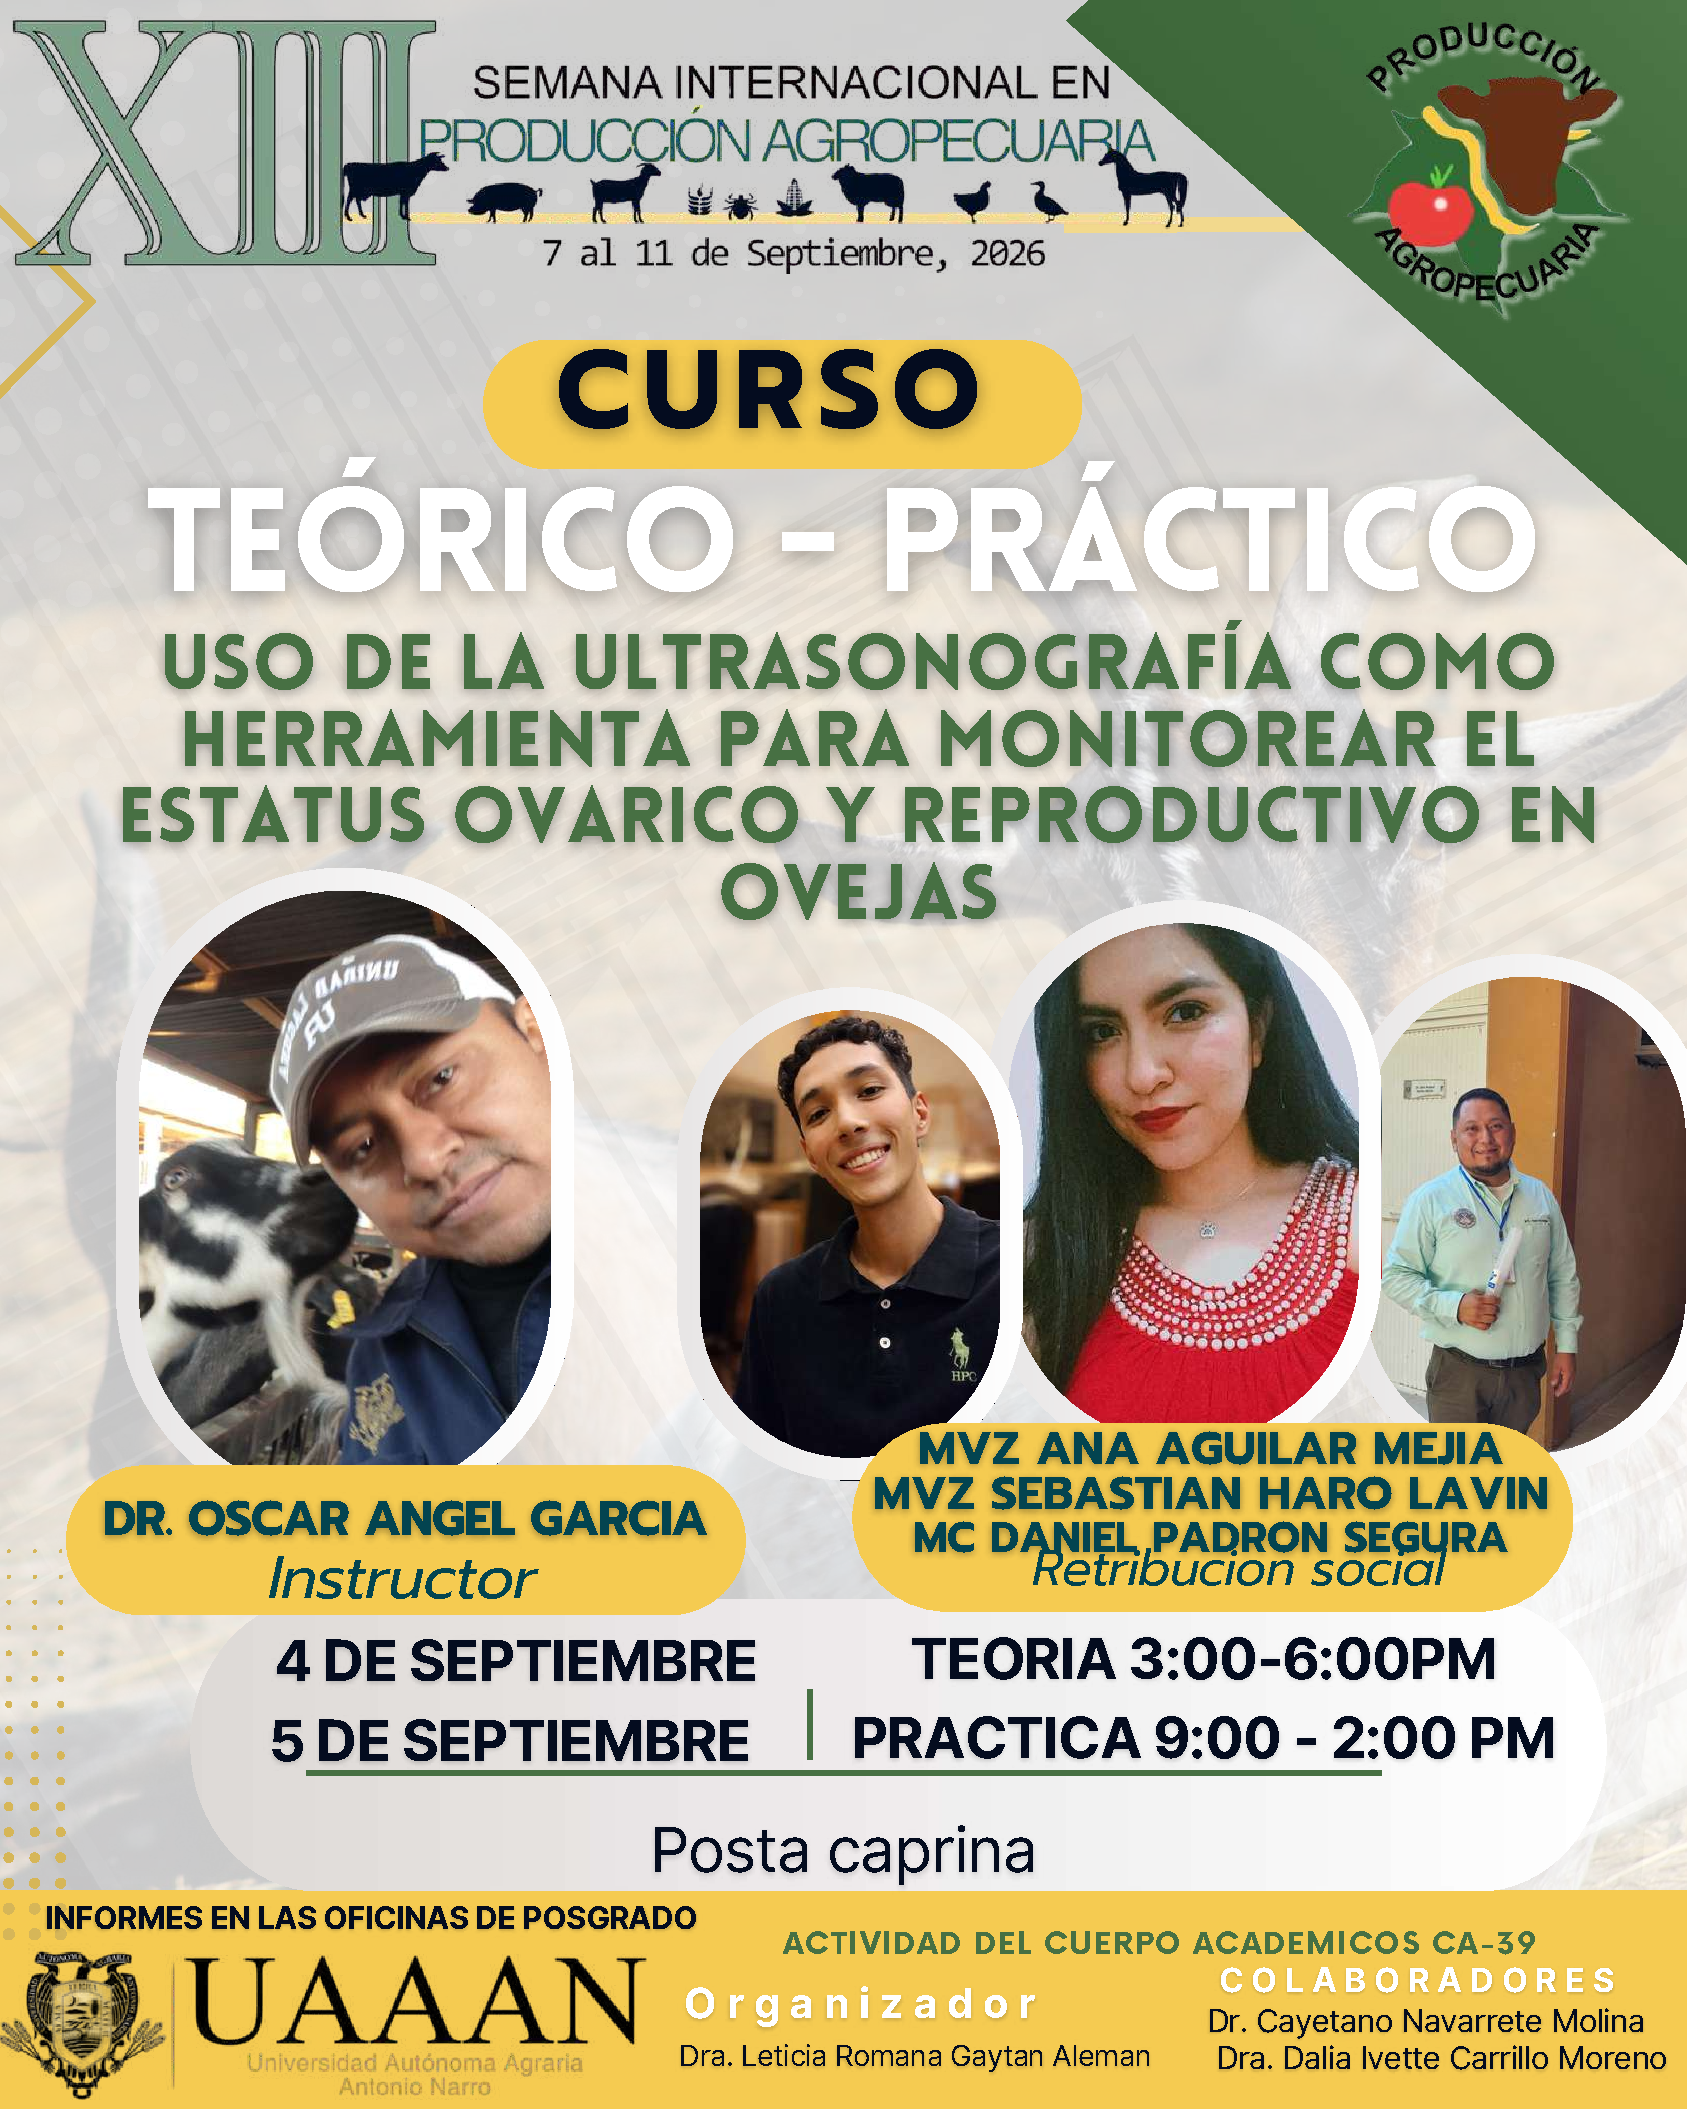
\includepdf[fitpaper=true,pages=-,width=\paperwidth]{images/events/sipa xiii course 1.pdf}
}

\newpage
\begin{wrap}
	\chapter{4 a 7 - Oscar}
	% If you're using TexStudio, this line helps you to identify the keynote/document/course in the editor's TOC
\end{wrap}
\cero
% Given that \pagenblanc{} is set in alone, here will appear the part title in the header instead of the abbreviated name
% In that case, you don't need to declare nombsec and abbrevnombs functions
%\nombsec{Uso de la ultrasonografía en ovejas -- Dr. Oscar Angel}% Custom section name
%\abbrevnombs{last names}{fist}{names}{}% In fact, you can completely omit this function until you allow it to appear again
\ijshortauthor{Dr. Oscar Angel García}% This function adds the name in the TOC
\author{%
	Dr. Oscar Angel García
}
\ijaffiliation{%
	Universidad Autónoma Agraria Antonio Narro, Unidad Laguna
}
\corresponding{}{}
\title{Uso de la ultrasonografía como herramienta para monitorear el estatus ovarico y reproductivo en ovejas}

\maketitle

\begin{minipage}{0.45\textwidth}
	\centering
	\textbf{Organizator}
	
	Dra. Leticia Romana Gaytán Alemán
	
	\textbf{Contributors}
	
	Dr. Cayetano Navarrete Molina
	
	Dra. Dalia Ivette Carrillo Moreno
	
\end{minipage}%
\hfil%
\begin{minipage}{0.45\textwidth}
	\centering
	\textbf{Social Compensation}
	
	MVZ. Ana Aguilar Mejía
	
	MVZ. Sebastián Haro Lavín
	
	M. C. Daniel Padron Segura
	
\end{minipage}

\begin{table}[H]
	\centering
	\begin{tabular}{c|c}
		\multicolumn{2}{c}{\textbf{Activities schedule}} \\
		\multicolumn{1}{c|}{\multirow{2}{*}{September 4 to 6}} & Theoretical course: \\
		\multicolumn{1}{c|}{} & 3:00 -- 6:00 pm \\
		\multicolumn{1}{c|}{\multirow{2}{*}{September 7 \& 8}} & Practical section: \\
		\multicolumn{1}{c|}{} & 9:00 am -- 2:00 pm
	\end{tabular}
\end{table}

% Here you can write the justification or introduction of the course/seminar/activity
\vspace{-.6cm}
\justify
Este curso de ultrasonografía clínica está dirigido a profesionales y estudiantes del área de veterinaria y zootecnia que deseen aprender a utilizar la ecografía como herramienta diagnóstica de manera segura, precisa y fundamentada en la práctica clínica.

% Here you can write the objective of the course/seminar/activity
\begin{center}
	\vspace{-.32cm}
	\textbf{Objetivo}
	\vspace{-.32cm}
\end{center}
\justify
El profesional o estudiante comprenderá los fundamentos de la ultrasonografía y el el uso de la ultrasonografía como una herramienta utilizada en tiempo real en el tracto reproductivo, monitorear la dinámica ovárica (folículos y cuerpos lúteos) y realizar un diagnóstico precoz y certero de la gestación, así como, patologías relacionadas con la reproducción.

\begin{center}
	\vspace{-.32cm}
	\textbf{Syllabus}
	\vspace{-.32cm}
\end{center}

\begin{enumerate}
	% If you only have the main activity names use -4pt of separation
	\setlength\itemsep{-4pt}
	\item Anatomía y fisiología del aparato reproductor de la hembra ovina
	\item Caracteristicas del ciclo reproductivo de la oveja
	\item Historia de la ultrasonografía en pequeños rumiantes
	\item Funcionamiento básico del ultrasonido
	\item Uso del ultrasonido en la dinámica ovárica
	\item Diagnostico de preñez en ovinos
	% If you have sub-activities use -10pt alongside the newer list
	%\setlength\itemsep{-10pt}
	%\begin{itemize}
	%	\vspace{-10pt}
	%	\setlength\itemsep{-4pt}
	%\end{itemize}
\end{enumerate}

% Pictures of the event
\begin{center}
	\vspace{-.32cm}
	\textbf{Photographic appendix}
	\vspace{-.32cm}
\end{center}

\rightimage{0.5}{images/course 1/sipa xiii im 1}{5.3}{1}{0.5}{Inauguración del curso por parte de\\ Dra. Viridiana Contreras Villarreal\\ Dra. Ma. Guadalupe Calderón Leyva y\\ Dra. Dalia Ivette Carrillo Moreno}

\leftimage{0.5}{images/course 1/sipa xiii im 2}{5.3}{1}{0.5}{Curso teórico por parte del\\ Dr. Oscar Angel García}

\newpage
\leftimage{0.5}{images/course 1/sipa xiii im 3}{8}{.8}{0.5}{Prácticas en las instalaciones de la Posta Caprina, UAAAN--UL}

\bigimage{images/course 1/sipa xiii collage}{20}{1}

\newpage
\begin{center}
	\vspace{-.32cm}
	\textbf{Commemorative photo of the course}
	\vspace{-.32cm}
\end{center}

\bigimage{images/course 1/sipa xiii final}{7}{1}

\newpage
% New course in a different page
{\hoffset=0pt

\includepdf[fitpaper=true,pages=-,width=\paperwidth]{images/events/sipa xiii course 2.pdf}
}

\newpage
\begin{wrap}
	\chapter{12 - blanca}
	% If you're using TexStudio, this line helps you to identify the keynote/document/course in the editor's TOC
\end{wrap}
\cero
% Given that \pagenblanc{} is set in yes, here will appear the section custom name in the header instead of the abbreviated name
% If you've already declared a section name, you can hide the function to leave it as it is
% If you want to change it, unhide the function and place another name
%\nombsec{Muestras en pequeñas especies -- M. C. Blanca Jimenez}% Custom section name
% For example, here is ommited the abbreviation function, as it's not necesary in this specific proceedings book
\ijshortauthor{M. C. Blanca Yaneth Jiménez Jiménez}% This function adds the name in the TOC
\author{%
	M. C. Blanca Yaneth Jimenéz Jimenez\textsuperscript{1}; M. C. Arturo Pacheco Luna\textsuperscript{2}
}
\ijaffiliation{%
	\textsuperscript{1}Universidad Autónoma Agraria Antonio Narro, Unidad Laguna; \textsuperscript{2}Universidad Autónoma Agraria Antonio Narro, Unidad Saltillo
}
\corresponding{}{}
\title{Toma de muestras en pequeñas especies}

\maketitle

% More information about the courses/seminars/activities
\begin{minipage}{0.45\textwidth}
	\centering
	\textbf{Organizator}
	
	Dra. Viridiana Contreras Villarreal
	
\end{minipage}%
\hfil%
\begin{minipage}{0.45\textwidth}
	\centering
	\textbf{Contributors}
	
	Dra. Dalia Ivette Carillo Moreno
	
	Dr. Alan Sebastián Alvarado Espino
	
\end{minipage}

\begin{table}[H]
	\centering
	\begin{tabular}{l|c}
		\multicolumn{2}{c}{\textbf{Activities schedule}} \\
		12 de septiembre & 10:00 am
	\end{tabular}
\end{table}

%For example, this course doesnt have any justification or introduction paragraph
\begin{center}
	\vspace{-.32cm}
	\textbf{Objetivo}
	\vspace{-.32cm}
\end{center}
\justify
Desarrollar en los estudiantes los conocimientos y habilidades básicas para la correcta toma, manejo y conservación de muestras sanguíneas, urinarias y fecales en perros y gatos, considerando los principios de bioseguridad y los factores que pueden afectar la calidad de las muestras y la confiabilidad de los resultados diagnósticos

% But this course established some specific objectives
\begin{center}
	\vspace{-.32cm}
	\textbf{Specific objectives}
	\vspace{-.32cm}
\end{center}
\begin{enumerate}
	\setlength\itemsep{-4pt}
	\item Comprender los principios fisiológicos y celulares involucrados en la criopreservación de espermatozoides equinos
	\item Identificar los principales factores que afectan la calidad seminal antes, durante y después de la congelación
	\item Conocer los métodos adecuados para la colección y manejo inicial del eyaculado
	\item Realizar una evaluación macroscópica y microscópica del semen fresco
\end{enumerate}

% The syllabus can have activities and sub-activities, though you can change it's format
\begin{center}
	\vspace{-.32cm}
	\textbf{Syllabus}
	\vspace{-.32cm}
\end{center}

\begin{multicols}{2}
	
	\begin{enumerate}
		% If you only have the main activity names use -4pt of separation
		%\setlength\itemsep{-4pt}
		% If you have sub-activities use -10pt alongside the newer list
		\setlength\itemsep{-10pt}
		\item Generalidades de la toma y manejo de muestras
		\begin{itemize}
			\vspace{-10pt}
			\setlength\itemsep{-4pt}
			\item Tipos de muestras biológicas
			\item Material y equipo básico
			\item Bioseguridad durante la toma y manejo de muestras
		\end{itemize}
		\item Muestras sanguíneas
		\begin{itemize}
			\vspace{-10pt}
			\setlength\itemsep{-4pt}
			\item Tubos de recolección y anticoagulantes
			\item Material para la venopunción
			\item Sitios de obtención de sangre
			\item Técnica básica de venopunción
			\item Manejo posterior a la toma
			\item Identificación y conservación
		\end{itemize}
		\item Muestras de orina
		\begin{itemize}
			\vspace{-10pt}
			\setlength\itemsep{-4pt}
			\item Métodos de obtención de muestras
			\item Material y recipientes
			\item Características de una muestra adecuada
			\item Identificación y conservación
			\item Tiempo y condiciones de almacenamiento
		\end{itemize}
		\item Muestras fecales
		\begin{itemize}
			\vspace{-10pt}
			\setlength\itemsep{-4pt}
			\item Características de una muestra adecuada
			\item Material y recipientes
			\item Métodos de recolección
			\item Identificación y conservación
		\end{itemize}
	\end{enumerate}
	
\end{multicols}

% Pictures of the event
\begin{center}
	\vspace{-.32cm}
	\textbf{Photographic appendix}
	\vspace{-.32cm}
\end{center}

\rightimage{0.5}{images/course 2/sipa xiii im 1}{5.3}{1}{0.5}{Presentación del curso a\\ los participantes}

\leftimage{0.5}{images/course 2/sipa xiii im 2}{5.3}{1}{0.5}{Presentación por parte de la\\ M. C. Blanca Janeth Jiménez}

\newpage

\images{0.5}{images/course 2/sipa xiii im 3}{5.3}{1}{0.5}{images/course 2/sipa xiii im 4}{8}{.8}

\begin{center}
	\vspace{-.32cm}
	\textbf{Foto conmemorativa del curso}
	\vspace{-.32cm}
\end{center}

\bigimage{images/course 2/sipa xiii final}{7}{1}


%=================================================
% Photographic  gallery
%=================================================
\newpage
\pagenblanc{alone}
\nombsec{}
\part{Photographic gallery}

\newpage
\nombsec{}

\vspace*{-0.7cm}
\phantomsection
\addcontentsline{toc}{section}{\hspace{-0.1cm}CONGRESS INAUGURATION}
\subseccion{Congress Inauguration}

\rightimage{0.5}{images/general/sipa xiii beggining}{5.3}{1}{0.5}{Inauguración del evento por parte del\\ Dr. Alejandro Moreno Resendez}

\vspace{-0.8cm}
\bigimage{images/general/sipa xiii collage}{17.3}{1}

% Photos day 1
\newpage
\vspace*{-0.7cm}
\phantomsection
\addcontentsline{toc}{section}{\hspace{-0.1cm}DAY 1}
\subseccion{Day 1}
\vspace*{\fill}
\vspace*{-0.5cm}
\bigimage{images/general/day 1/sipa xiii 1}{21}{1}
\vspace*{\fill}

\newpage
\vspace*{\fill}
\bigimage{images/general/day 1/sipa xiii 2}{21}{1}
\vspace*{\fill}

% Photos day 2
\newpage
\vspace*{-0.7cm}
\phantomsection
\addcontentsline{toc}{section}{\hspace{-0.1cm}DAY 2}
\subseccion{Day 2}
\vspace*{\fill}
\vspace*{-0.5cm}
\bigimage{images/general/day 2/sipa xiii 1}{21}{1}
\vspace*{\fill}

\newpage
\vspace*{\fill}
\bigimage{images/general/day 2/sipa xiii 2}{21}{1}
\vspace*{\fill}

\newpage
\vspace*{-0.7cm}
\subseccion{Thank you for attending}
\vspace*{-0.5cm}
\bigimage{images/general/sipa xiii final}{8}{1}


% Bibliographic content page
\newpage
\pagestyle{plain}
\vspace*{.2cm}
\fontsize{10}{11}\selectfont
\setlength{\parindent}{0pt}
Original title:

Title: Subtitle\\

1st volume

1$^{\text{st}}$ edition  --- october 12, 2026\\

\textbf{Proceedings' organizing and supervisory committee}

\setlength{\columnsep}{0pt}
\begin{multicols}{2}
\centering
Lic. Francisco Gerardo Véliz Romero

Lic. Francisco Gerardo Véliz Romero

Lic. Francisco Gerardo Véliz Romero

Lic. Francisco Gerardo Véliz Romero
\end{multicols}

\copyright\, Francisco Gerardo Véliz Romero

\copyright\, Of the texts and images, their respective authors\\

Coder design: Lic. Francisco Gerardo Véliz Romero, based on the VIII Semana Interancional en Producción Agropecuaria's cover

Document design and compilation: Lic. Francisco Gerardo Véliz Romero\\

This publication includes the keynote lectures of the speakers invited to the event, the abstracts of the posters shown by the master's and doctoral students of the Agricultural Production Science Postgraduate Program, as well as the discussion's program and the participants's biographies, and the information about the courses offered during the event

The document's code was elaborated by Lic. Francisco Gerardo Véliz Romero, and the document itself was compiled employing the TeXworks program.

The conference proceedings template can downloaded in: 

\faGithub\, \url{https://github.com/francisco-veliz-romero/XIII-SIPA-Proceedings}\\

Disclaimer: The opinions, interpretations, results, and conclusions expressed in the contributions to this volume belong to their respective authors, and do not necessarily represent the opinions of the organizers or participating institutions. The editors and organizers assume no responsibility for any use that may be made of the information presented in this volume\\

Suggested citation format for this book:

Navarrete-Molina, C., \& Véliz-Romero, F. G. (Eds.) (2026). \textit{Proceedings of the XIII International Week on Agricultural Production: Keynote lectures, summaries, courses and discussion forum} (1st ed., Vol. 1, p. 135). Torreón, Coahuila, México. \url{https://www.researchgate.net/publication/415049442_Memorias_de_la_XIII_Semana_Internacional_en_Produccion_Agropecuaria}

Formato de cita sugerida para algún documento incluido en este libro:

\textbf{Author's names} (2026). \textbf{Title}. In: Navarrete-Molina, C., \& Véliz-Romero, F. G. (Eds.) \textit{Proceedings of the XIII International Week on Agricultural Production: Keynote lectures, summaries, courses and discussion forum} (1st ed., Vol. 1, \textbf{page numbers}). Torreón, Coahuila, México. \url{https://www.researchgate.net/publication/415049442_Memorias_de_la_XIII_Semana_Internacional_en_Produccion_Agropecuaria}

\end{document}
